\section{Data}
\label{sec:data}

\paragraph{Source and period.}
All data in the main experiments come from a public corpus of pump.fun activity collected continuously from websocket feeds and Solana RPC polling between 5 June and 14 July 2026~\citep{slinkdev2026corpus}. It covers 798,430 token launches and 33.6 million trades on the bonding curve. Following the corpus documentation, we exclude trade rows attributed to the Solana System Program address, which is not a market participant; this leaves 26.9 million trade events. The corpus records no trades on 3 July 2026 because of a collection outage, and labels whose windows touch that day are treated as unavailable. Some tokens' trades carry no price; their surge labels are unavailable as well. Market-wide context features are computed from the same corpus. We stored every extract with checksums and froze the full dataset before training any model.

\paragraph{Population.}
Of the 798,430 launches, 622,303 tokens have at least one trade on the curve, and these form our modeling population. The primary detector finds a surge in 49,836 of them.

\paragraph{Observation sampling.}
We observe each token at fixed ages (launch, 10\,s, 30\,s, 1\,min, 2\,min, 5\,min, 10\,min, 30\,min, 1\,h and 6\,h) and at the moment of its $k$-th trade for $k \in \{1, 2, 4, \ldots, 512\}$. Both rules use only information available at the observation time: fixed ages depend only on the launch time, and the $k$-th trade has, by definition, already happened. Coincident observations are de-duplicated. This yields 8,449,949 observations. The scheme gives every token the same set of fixed-age observations, and gives active tokens extra observations exactly when trading picks up, which is when surges tend to start.

\paragraph{Splits.}
We split tokens chronologically by launch time, using quantiles of the launch-time distribution. Tokens launched before 1 July 2026, 01:34~UTC (the 70th percentile) form the training set; tokens launched between that point and 7 July 2026, 21:19~UTC (the 85th percentile) form the validation set; later tokens form the test set. Splits are token-disjoint, and tokens with identical launch timestamps stay on the same side of each boundary. Inside the training period we define two walk-forward folds for model selection: fold~1 trains on tokens launched before the 40th percentile and validates on the 40th to 55th percentiles; fold~2 trains before the 55th percentile and validates on the 55th to 70th. Every hyperparameter, number of boosting rounds and baseline choice was made on these folds. Table~\ref{tab:data} and Figure~\ref{fig:timeline} summarize the data.

\begin{table}[t]
\centering
\caption{Data summary. Base rates are the share of eligible observations whose token begins a primary-definition surge within the horizon.}
\label{tab:data}
\tabsize
\begin{tabular}{lrrr}
\toprule
 & Train & Validation & Test \\
\midrule
First launch (2026, UTC) & 5 Jun 09:12 & 1 Jul 01:34 & 7 Jul 21:19 \\
Last launch (2026, UTC) & 1 Jul 01:34 & 7 Jul 21:19 & 14 Jul 15:01 \\
Tokens with $\geq$1 trade & 435{,}612 & 93{,}345 & 93{,}346 \\
Observations & 5{,}879{,}063 & 1{,}275{,}120 & 1{,}295{,}766 \\
Primary surges with onset in window & -- & 9{,}182 & 12{,}225 \\
Base rate, onset within 60 s & -- & 1.78\% & 2.29\% \\
Base rate, onset within 300 s & -- & 2.11\% & 2.73\% \\
\bottomrule
\end{tabular}

\end{table}

\begin{figure}[t]
\centering
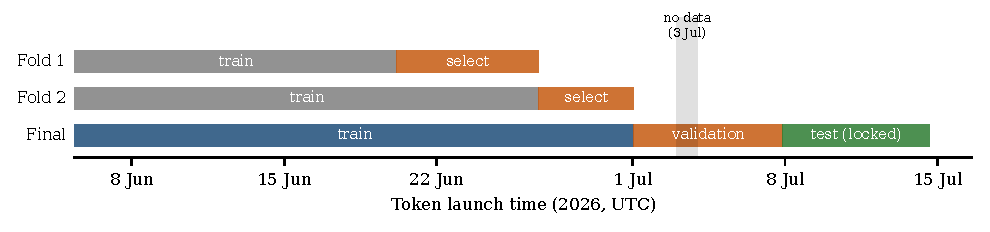
\includegraphics[width=\linewidth]{figures/fig_timeline.pdf}
\caption{Chronological splits. Walk-forward folds inside the training period were used for every model choice; the validation week was used for development reporting; the test week was scored once under a preregistered protocol. The corpus has no trades on 3 July 2026.}
\label{fig:timeline}
\end{figure}
